\chapter{Hintergrund}

Dieses Kapitel legt den Grundstein für diese Arbeit. Es liefert den theoretischen Hintergrund, sowie die Motivation für die Forschung zur Digitalisierung im Handwerk. Zuerst wird der Stand der Digitalisierung in Handwerksbetrieben, sowie kleinen und mittleren Unternehmen dargelegt, welcher Anreiz gegeben hat, dieses Thema genauer zu beleuchten. Anschließend wird herausgearbeitet, wie digitale Anwendungen bereits eingesetzt werden, um bei bestimmten Arbeitsschritten zu unterstützen. Dabei werden Spezifikationserstellung und Dienstleistungsunterstützung genauer betrachtet und mit Beispielen veranschaulicht. Zuletzt wird auf das Potenzial von Augmented Reality zur Visualisierung eingegangen und dies wiederum durch Beispielanwendungen veranschaulicht.

\section{Digitalisierung in Handwerksbetrieben, kleinen und mittleren Unternehmen}

Die Digitalisierung hält Einzug in den meisten Branchen, was in dieser modernen Zeit, in welcher auch im privaten Leben mehr und mehr Technik zum Einsatz kommt, nicht verwunderlich ist. Mithilfe neuer Technologien und Programmen lassen sich beispielsweise Abläufe beschleunigen, Genauigkeit und Effizienz verbessern, sowie die Erreichbarkeit steigern. Oft werden diese Technologien zum bewältigen des Verwaltungsaufwands genutzt, was kleinen und mittleren Unternehmen (\textbf{KMUs}), als auch Handwerksbetrieben mehr Zeit für ihre eigentliche Aufgabe lässt: das Handwerk \cite{noauthor_neue_nodate}. Unternehmen wollen sich diese neuen Chancen zu nutze machen und Investieren dazu in Umrüstung und Umstrukturierung von Unternehmensabläufen, sowie in die Integration von neuen Programmen und technischen Hilfsmitteln in ihr Arbeitsumfeld \cite{TODO: Buchkapitel}. Große, kommerzielle Unternehmen fällt das leichter als KMUs und Handwerksbetrieben \cite{hateful_six_krcmar}.

KMUs spielen aber ein wichtige Rolle in unserer Gesellschaft und Wirtschaft, weshalb ihr langsamer Fortschritt im Bereich Digitalisierung auf keinen Fall leicht zu nehmen ist. In den USA beispielsweise stellen KMUs 95\% aller Unternehmen und sind verantwortlich für zwei Drittel aller neuen Arbeitsplätze. Zusätzlich werden 60\% des Exports von ihnen gestemmt \cite{allocca_innovation_2006}. Diese Argumente machen KMUs zu einem lohnenswerten und interessanten Forschungsgebiet, was sich in den letzten Jahren auch deutlich zeigte.

Fries et al. \cite{hateful_six_krcmar} trug durch ihre Forschung sechs Faktoren zusammen, welche dafür verantwortlich sind, dass KMUs ihren größeren Konkurrenten in der Digitalisierung hinterher hängen. Das liegt an: 

\begin{enumerate}
	\item einem empfundenen Ungleichgewicht zwischen Risiken und Möglichkeiten,
	\item mangelnder Vereinbarkeit mit der täglichen Arbeitsroutine,
	\item einer schwierigen Eingliederung in individuelle Geschäftsprozesse,
	\item komplexen Infrastrukturinvestitionen,
	\item nicht oder kaum vorhandenem IT Knowhow und
	\item hohen Installationskosten für die Inbetriebnahme der neuen Technologien.
\end{enumerate}

KMUs denken bei dem Einsatz von neuen Technologien vermehrt an Risiken und Kosten, als an Chancen, die daraus entstehen oder andere positive Aspekte. Sie haben limitierte Ressourcen an Kapital und Arbeitskräften und können sich daher keine falschen Entscheidungen oder Investitionen erlauben \cite{allocca_innovation_2006}. Mit dem Adaptieren und Einsatz von Innovationen geht immer ein hohes finanzielles Risiko einher. KMUs können, im Gegensatz zu größeren Firmen, diese Kosten meist nicht über mehrere Projekte verteilen, um die Belastung zu minimieren \cite{rothwell_small_1989}. \\
Alloca und Kessler \cite{allocca_innovation_2006} wiederum schreiben KMUs mehr Risikobereitschaft zu, da das Management bzw. die Geschäftsführung meist aus Entrepreneurs besteht, die den Einstieg in die Industrie durch Wagnisse schaffen wollen oder geschafft haben. Ein solches Unternehmen muss, aufgrund der knapperen Ressourcen, schneller und effizienter arbeiten, um konkurrenzfähig zu bleiben.

Des weiteren spielt es eine große Rolle, ob neue Technologien den Arbeitsalltag tatsächlich erleichtern und wie diese von den Mitarbeitern aufgenommen und in ihre Routine integriert werden. Dies kann besonders bei älteren Mitarbeitern, die \textit{"schon immer so gemacht"} haben schwierig werden. Die Arbeitsprozesse müssen umgebaut werden, um die neuen Geräte oder Programme zu unterstützen und ihre Potential zu nutzen. Da oft niemand vorhanden ist, der sich ausschließlich mit \textit{Research \& Development} beschäftigt, sind diese Entscheidungen schwer zu treffen \cite{rothwell_small_1989}. Nichtsdestotrotz haben KMUs aufgrund weniger Bürokratie das Potenzial, schneller Änderungen zu adaptieren (\cite{kessler_innovation_1996} und \cite{kessler_speeding_1999}, zitiert in \cite{allocca_innovation_2006}).

Unternehmerische Manager können oft die steigende Komplexität der Firma, durch deren Wachstum und Integration von neuen Technologien, schwer überblicken, worunter die Eingliederungen von Neuerungen in Geschäftsprozesse leidet \cite{rothwell_small_1989}. Dafür sind weniger standardisierte Prozesse und Guidlines, ein weniger systematischer Management Style und generell die geringere Erfahrung des Managements im Vergleich zu großen Unternehmen verantwortlich \cite{allocca_innovation_2006}. 

Das Einbinden der neuen Technologien in die bestehende Infrastruktur des Unternehmens stellt zusätzliche Risiken und Kosten dar. Der Arbeitsplatz war meist ursprünglich nicht dafür designed, um schnell und einfach neue Geräte oder Programme zu integrieren. Teilweise lässt auch der Ort an dem gearbeitet wird den Einsatz generell nicht oder nur bedingt zu. Auf einer Baustelle oder in einem Kellergewölbe beispielsweise kann keine permanente WLAN Verbindung sichergestellt werden \cite{TODO: Buchkapitel}. Dadurch wird der Einsatz von digitalen Medien erschwert.

Da KMUs und vor allem Handwerksbetriebe oft aus wenigen Mitarbeitern bestehen, ist die Wahrscheinlichkeit hoch, dass kein Technikspezialist an Board ist. Das macht es nötig, sich fremde Expertise einzuholen, um in die richtige Technologie für den Betrieb zu investieren. Jedoch bringt das zusätzliche Kosten und Zeitaufwand mit sich, welche oft nicht verfügbar sind \cite{rothwell_small_1989}. Des weiteren müssen die Mitarbeiter für die neue Technologie geschult werden, wodurch wieder Zeit verloren geht. Fehler, die durch Anschaffung falscher technischer Hilfsmittel, oder durch unsachgemäßen, ineffizienten Einsatz dieser entstehen, kosten unnötig Geld. Das kann sich ein Unternehmen mit begrenzten Ressourcen nicht leisten \cite{allocca_innovation_2006}.

Die Schulung der Mitarbeiter ist durchaus zeit- und kostenaufwändig. Aber auch die Anschaffung und Installation der neuen Technologie birgt eine finanzielle Hürde für die Unternehmen. Zusätzliche, versteckte Kosten welche durch Probleme mit Patenten oder Auflagen des Staates entstehen, stellen eine große Belastung bei der Integration dar \cite{rothwell_small_1989}. 

Trotz dieser Hindernden Faktoren für KMUs und Handwerksbetriebe bieten sich viele Möglichkeiten für diese. Ritchie und Brindley \cite{ritchie_ict_2005} sehen großes Potential für diese Unternehmen im Bereich Digitalisierung mit ihren kommerziellen Konkurrenten mitzuhalten, da sie \textit{flexibler, effizienter und adaptiver} sind, was Grundvoraussetzungen für die Integration von Neuerungen ist. \\
Das bereits Produkte zur Unterstützung für Handwerksbetriebe und KMUs existieren und genutzt werden, wird im Folgenden genauer dargestellt.

\section{Unterstützung der Spezifikationserstellung mit digitalen Anwendungen}
\label{sec:spezi}

''Auf Baustellen müssen sich Kunde und Handwerker erst einig werden, was genau getan werden soll, denn ''[g]erade im Dienstleistungsbereich gibt es einen engen Zusammenhang zwischen hoher Kundenzufriedenheit und dem Einbinden des Kunden''.'' (\cite{TODO: Buchkapitel}, zitiert nach \cite{hentrich_arbeiten_2002}). Die Kommunikation des Plans gestaltet sich dabei oft schwierig. Ein Problem, das viele Handwerker anmerken (siehe Fokusgruppe \ref{sec:fokus}) ist, dass Kunden wenig Vorstellungsvermögen haben. Der Handwerker, als Experte, kann einen Raum betreten und sich direkt vorstellen, wie er diesen gestalten würde. Dies dem Kunden nur durch Worte zu kommunizieren ist jedoch schwierig. Dadurch kann der Handwerker den Kunden nicht effektiv beraten und dieser kann wiederum schwer seine Vorstellungen beschreiben. Verschiedene Werkzeuge können dabei helfen, dies zu veranschaulichen.

Traditionell werden Baupläne und Blaupausen auf Papier in 2D gezeichnet \cite{TODO: Buchkapitel}. Der technische Zeichner kann so ganze Gebäude bis ins kleinste Detail spezifizieren und sogar mit Inneneinrichtung ausstatten. Diese Methode hat jedoch zum Nachteil, dass zum Lesen der Pläne sehr viel Erfahrung erforderlich ist. Gleichzeitig sind diese, aufgrund ihrer Komplexität, auch für erfahrene Handwerker fehleranfällig und führen zu Fehlern bei der Umsetzung \cite{wang_using_2007}. Für den Kunden bringt die Verwendung dieser Pläne kaum einen Vorteil bezüglich des Verständnisses. Die Zeichnungen sind technisch komplex, können von Laien nur mäßig verstanden werden und tragen dadurch nur mäßig zu einer besseren Kunde-Handwerker-Kommunikation bei.

Es wird also ein Mittel oder Werkzeug benötigt, dass diese Verständigung und somit auch die Spezifikation und den Vertragsschluss unterstützt. Es soll dabei den Kunden unterstützen die Pläne des Handwerkers besser zu verstehen und sich vorstellen zu können. Dafür muss es geeignete Visualisierungsmethoden mitbringen, um den Plan verständlich darzustellen. \\
Der Kunde kann anhand des ihm gezeigten Bildes besser Änderungen Vorschlagen. So kann er deutlicher Änderungsvorschläge bringen, zeigen wo er sie Anbringen möchte und erleichtert damit das Kundengespräch für beide Parteien. \\
Es ermöglicht auch dem Handwerker einfach verständlicher Ratschläge zu geben und gezielt auf Details einzugehen. Dies steigert zusätzlich die vom Kunden empfundene Kompetenz des Handwerkers, da er direkt sehen kann, was die Pläne des Handwerkers sind und sich besten Fall vorstellen kann, wie das Endergebnis aussieht. \\
Anschließend werden einige, teils kommerzielle, Spezifikationswerkzeuge vorgestellt, die diesen Zielen genügen.

\begin{figure}[H]
	\begin{center}
		\includegraphics[scale=0.65]{Resources/Hintergrund/sketchup.jpg}
		\caption{3D Modellierter Bauplan in SketchUp 3D}
	\end{center}
\end{figure}

SketchUp 3D ist eine 3D-Modellierungssoftware, die 2D hand- oder computergezeichnete Baupläne zugänglicher machen kann. Dazu ermöglicht es die teilweise Umwandlung dieser 2D Zeichnungen in 3D Modelle. Bilder werden in SketchUp eingefügt, mit zusätzlichen Informationen versehen und erweitert. Eine der Funktionalitäten ist es beispielsweise eine Wand zu markieren und diese ''aus der Zeichnung heraus zu ziehen''. So erstellt das Programm ein 3D Modell des Raums, durch das sie der Kunde am Computer bewegen kann. Gleiches kann auf Tische und Ähnliches angewandt werden. Zusätzlich ist es möglich, Texturen auf Objekte zu legen. Der Nutzer kann damit den Wänden die Farbe geben, die der echte Raum hat, oder mit verschiedenen Designs experimentieren, um seine gewünschte Stimmung zu erhalten. Dadurch bekommt der Kunde ein Gefühl dafür, wie das Endergebnis aussehen kann. \\
Robert M. Wolk \cite{wolk_utilizing_2008} nutzt SketchUp 3D in Kombination mit Google Earth, um Bürgern mehr Mitbestimmungsrecht bei der Planung eines Windparks zu geben. Dafür erstellt er den Windpark in SketchUp und fügt diesen in Google Earth an der geplanten Bauposition ein (siehe Abbildung \ref{windfarm}). Die Bürger können diesen nun über Google Earth aus ihrer eigenen Perspektive betrachten und abwägen, welche Auswirkungen dieser auf ihr zu Hause oder ihren Arbeitsplatz haben wird. Dadurch können sie eine besser fundierte Entscheidung treffen, ob sie dafür oder dagegen sind.

\begin{figure}[h]
	\begin{center}
		\noindent\includegraphics[scale=0.6]{Resources/Hintergrund/Windfarm.jpg}
		\label{windfarm}
		\caption{Windfarm Modell in Google Earth}	
	\end{center}
\end{figure}

\begin{figure}[h]
	\begin{center}
		\noindent\includegraphics[scale=0.2]{Resources/Hintergrund/irisVR.jpg}
		\label{irisVR}
		\caption{Kollaboration in irisVR an 3D Modell}	
	\end{center}
\end{figure}

Mit irisVR können Designer ihre, am PC erstellten, Blaupausen und 3D Modelle in Virtual Reality (VR) betrachten. Kunden oder Designer können sich dann, mit Hilfe einer VR-Brille, frei in diesem Raum bewegen. Dadurch, dass er das Objekt von allen Seiten betrachten kann bekommt der Kunde eine gute Vorstellung davon. Außerdem kann der Kunde mit dem Modell in VR interagieren. Mehrere Personen können gleichzeitig per VR auf das Modell zugreifen, es bearbeiten und so über Änderungen kommunizieren (siehe Abbildung \ref{irisVR}). Teilweise ist es möglich 3D Modelle in AR mit Hilfe von Tablets oder Smartphones zu betrachten. Ein Raum, in welchem Objekte abgebildet werden sollen, muss davor genau abgemessen und im Modelling Programm angelegt werden. Objekte die jetzt darin positioniert werden, erscheinen als Hologramme am Tablet in den entsprechenden Positionen. 3D Modelle können aus verschiedenen Design Softwarelösungen eingelesen werden. Momentan unterstützt irisVR beispielsweise Revit, SketchUp, OBJ, Grasshopper oder Rhino \cite{helander_joel_2017}. 

Ein weiteres Werkzeug, welches sehr Kundenbezogen ist, ist der Küchenplaner von Biller. Dieser unterstützt am besten, wenn der Grundriss des Raumes, in welchem eine Küche eingebaut werden soll, bekannt ist, der Kunde jedoch noch keine Vorstellung hat, wie seine Küche aussehen bzw. kosten soll. Er kann die Maße und Wandfarben \enquote{genau wie daheim} setzen und den Raum mit Elementen bestücken. Der Küchenplaner errechnet selbst passende Küchenkombinationen als Vorschläge für diesen Raum, sodass nicht alles von Hand positioniert werden muss. Diese Vorschläge können betrachtet und den Wünschen entsprechend angepasst werden. Gleichzeitig zeigt der Planer Preise an und es können Vorschläge aus verschiedenen Preissegmenten gewählt werden.

\begin{figure}[H]
	\begin{center}
		\noindent\includegraphics[scale=0.5]{Resources/Hintergrund/biller.png}
		\caption{Biller Küchenplaner mit Anpassungsmöglichkeiten}	
	\end{center}
\end{figure}

\begin{figure}[h]
	\begin{center}
		\noindent\includegraphics[scale=0.4]{Resources/Hintergrund/schedule4D.png}
		\caption{Schedule Simulator: Modell und Zeitplan}	
	\end{center}
\end{figure}

Die allseits bekannten und weit verbreiteten CAD Systeme dürfen in dieser Aufzählung natürlich nicht fehlen. Mit Schedule Simulator, einem 4D CAD System, hat Bentley Systems das klassische CAD um eine weitere Dimension erweitert. Damit ist es möglich eine gesamte Baustelle, mit Hauptaugenmerk auf zeitlicher Strukturierung, planen. Der Bauleiter legt damit fest, welche Arbeitsschritte nacheinander ausgeführt werden müssen und Schedule Simulator zeigt ihm dazu ein visuelles Modell der einzelnen Bauphasen. Dafür können 3D Modelle aus verschiedenen CAD Programmen geladen werden. An diese werden Zeitplanungsdaten angehängt und das Programm erstellt daraus eine 4D Simulation der Baustelle und der einzelnen Arbeitsschritte \cite{heesom_trends_2004}. Dadurch hat der Bauleiter den gesamten Zeitplan im Blick und kann schnell Änderungen vornehmen, falls sich etwas verzögert. Gleichzeitig kann er dem Kunden den aktuellen Fortschritt zeigen und weitere Schritte erklären. Das unterstützt bereits bei der Vertragsschließung, da alle Vorgänge genau spezifiziert werden können.

\begin{figure}[h]
	\begin{center}
		\noindent\includegraphics[scale=0.4]{Resources/Hintergrund/paletteSlider.png}
		\label{fotoreal}
		\caption{PaletteCAD: Planungsansicht und Fotorealistik Optik}	
	\end{center}
\end{figure}

Ein weiteres Werkzeug aus dieser Gruppe ist das Inneneinrichtungstool PaletteCAD. Damit lassen sich ganze Zimmer planen, wie beispielsweise ein Bad mit Dusche, Badewanne, etc.. Hauptsächlich wird es von Fliesenlegern und Schreinern verwendet. Das Programm liefert eine riesige Auswahl an Material, wie z.B. Fliesen, welches direkt aus den Datenbanken der Hersteller bezogen und regelmäßig geupdated wird. Die designten Räume können anschließend in Fotorealistik Optik gerendert werden (siehe Abbildung \ref{fotoreal}). Zusätzlich lassen sich Modelle für Schreiner direkt auf eine CNC Maschine übertragen. Die Macher versprechen durch benutzerfreundliches Design eine drastische Zeitersparnis bei der Planung.

\section{Augmented Reality als Visualisierungswerkzeug}

In der Allgemeinheit ist VR schon länger bekannt und verbreitet. Dabei wird der Nutzer aus der Realität in eine virtuelle Welt versetzt und nimmt seine physikalische Umgebung nicht mehr war. Momentan wird diese Technologie hauptsächlich für Computerspiele und Filme genutzt, was sie kommerziell, für private Anwender interessant macht. Zur Unterstützung bei der Arbeit wird VR aber auch teilweise schon als Visualisierungstool genutzt. \\
Augmented Reality hingegen hat den Vorteil, dass der Nutzer nicht in eine virtuelle Welt versetzt wird, sondern seine physikalische Umgebung noch wahrnimmt. Dies wird durch ein transparentes Display der Datenbrille, wie beispielsweise der Microsoft HoloLens gewährleistet. AR bietet die Möglichkeit die reale Welt durch Hologramme zu erweitern. Es werden Texte und Objekte in die Umgebung des Nutzers projiziert, mit denen er interagieren kann. Daher ist AR als Visualisierungswerkzeug, vor allem in realen Szenarien bestens geeignet. Es kann dabei unterstützen sich Modelle oder Zusammenhänge besser Vorzustellen, da man damit im realen Raum agieren und sie von allen Seiten betrachten kann.

TĂBUȘCĂ \cite{tabusca_augmented_2014} zeigt in seiner Arbeit verschiedene AR Applikationen, welche als Visualisierungswerkzeuge genutzt werden. \\
Eine interessante Applikation aus dem Einzelhandel, welche den Kunden bei der Entscheidungsfindung unterstützen soll, ist \textit{The Sampler} von Converse. Sie ermöglicht es dem Nutzer Schuhe bequem zu Hause \enquote{anzuprobieren} und so zu prüfen, ob ihm das Design gefällt. Dafür richtet er seine Smartphone oder Tablet Kamera auf seinen Fuß. Der Schuh wird dann darauf projiziert. Die Applikation ermöglicht dem Nutzer auch mit verschiedenen Farben und Designs zu experimentieren, um so den passenden Schuh für ihn zu finden und ihm bei der Entscheidungsfindung zu assistieren.

\begin{figure}[h]
	\begin{center}
		\noindent\includegraphics[scale=0.45]{Resources/Hintergrund/sampler.jpg}
		\caption[The Sampler von Converse]{The Sampler von Converse\footnotemark}	
	\end{center}
\end{figure}

\footnotetext{Quelle: \url{https://www.webbyawards.com/winners/2011/advertising-media/individual/augmented-reality/converse-the-sampler/} vom 04.01.2019}

IBM entwickelte 2013 auch eine App für den Einzelhandel, speziell für Lebensmittel in den USA. Dabei verwendet der Nutzer sein Smartphone oder Tablet beim Lebensmitteleinkauf, um zusätzliche Informationen zu erhalten. Er richtet die Kamera auf ein Regal und bekommt Optionen eingeblendet, mit denen er sich zusätzliche Informationen, wie zum Beispiel das Herkunftsland anzeigen lassen kann. Die Applikation erlaubt es auch Filter zu verwenden und so das Sortiment beispielsweise nur nach veganen oder glutenfreien Produkten zu durchforsten.

\begin{figure}[h]
	\begin{center}
		\noindent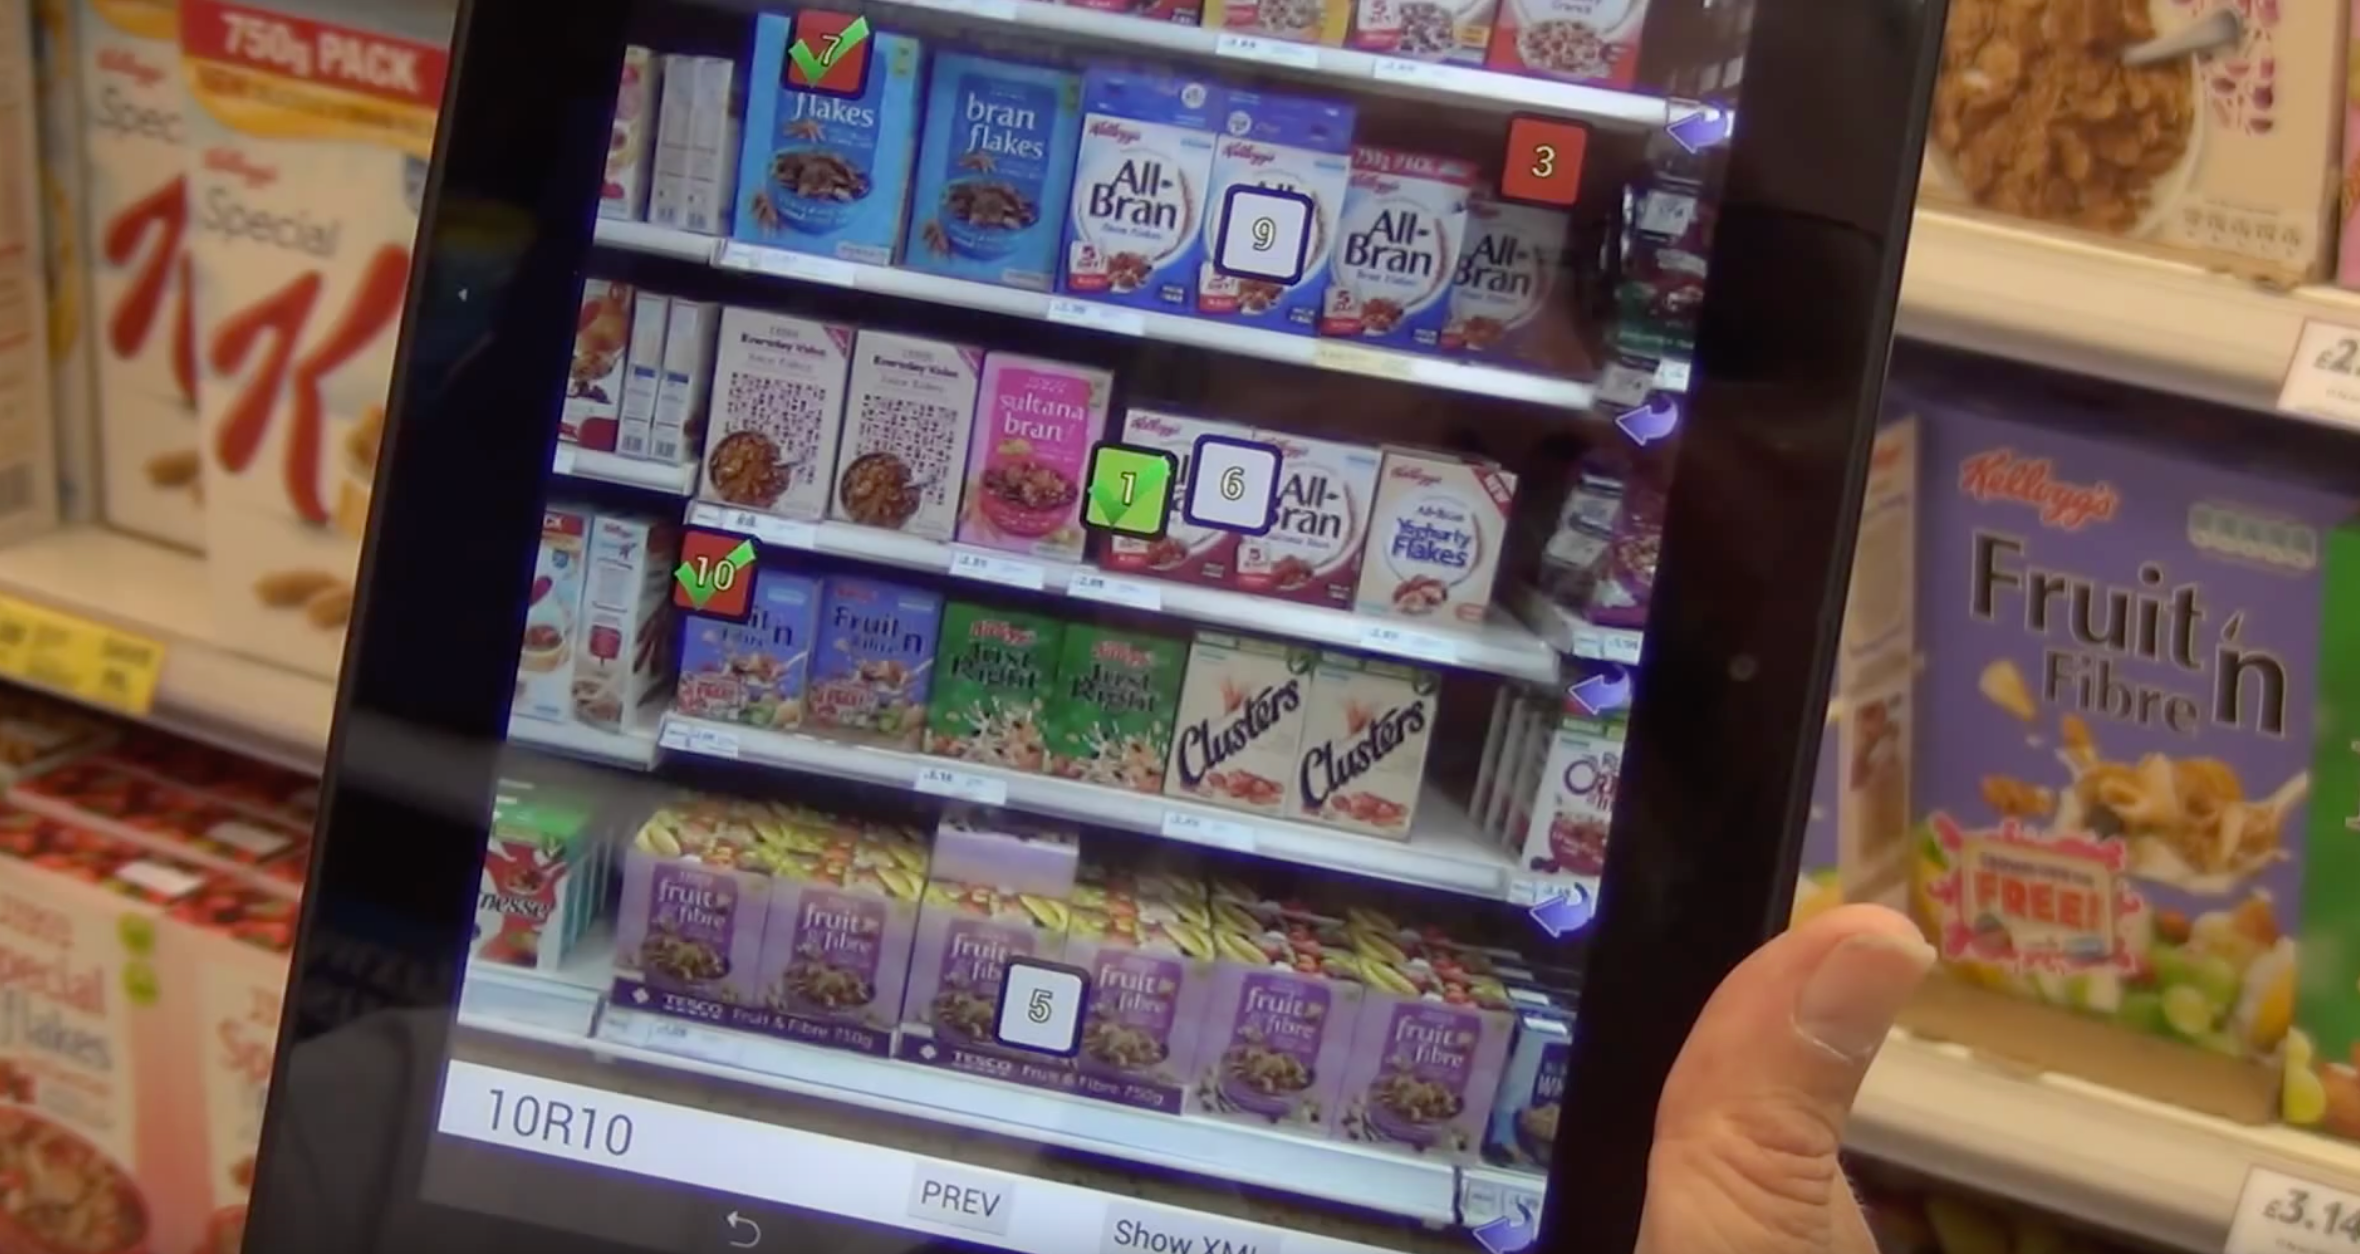
\includegraphics[scale=0.35]{Resources/Hintergrund/IBM.png}
		\caption[IBM Shopping App]{IBM Shopping App\footnotemark}	
	\end{center}
\end{figure}

\footnotetext{Quelle: \url{https://busy.org/@billigeplaetze/3waystodoaugmentedrealitywrong-3e0y2hze7f} vom 04.01.2019}

Auch IKEA nutzen die Möglichkeiten von AR in ihrer IKEA Place App zur Unterstützung bei Kaufentscheidungen. Die Applikation lässt den Nutzer Möbelstücke virtuell im physikalischen Raum positionieren. Er wählt ein Möbelstück aus dem Katalog und richtet seine Kamera auf die gewünschte Position dafür im Raum. Auf dem Display, zwischen den physikalischen Möbeln, erscheint nun ein virtuelles Modell des Möbelstücks in Originalgröße. Die Farben werden sogar an die Lichtverhältnisse angepasst. Der Nutzer kann das Möbelstück aus allen möglichen Blickwinkeln betrachten, wodurch er eine bessere Kaufentscheidung treffen kann und sich viel Zeit und Geld spart \cite{helander_joel_2017}.

\begin{figure}[h]
	\begin{center}
		\noindent\includegraphics[scale=0.4]{Resources/Hintergrund/ikea.jpg}
		\caption[IKEA Place App]{IKEA Place App\footnotemark}	
	\end{center}
\end{figure}

\footnotetext{Quelle: \url{https://mashable.com/2017/09/24/download-this-ikea-place-ar-kit-app/?europe=true##5LARqrPSqiqW} vom 04.01.2019}

Xiangyu Wang \cite{wang_using_2007} beschreibt in seiner Arbeit, wie man einen Bauleiter mit AR beim planen einer Baustelle unterstützen kann. Dieser kann mit der von Wang implementierten AR Applikation den gesamten Aufbau der Baustelle planen und visualisieren. 3D Objekte von Baustellenobjekten (siehe Abbildung \ref{bauModelle}), wie beispielsweise Kräne oder Bagger, können auf einer virtuellen Abbildung der Baustelle, welche der Nutzer vor sich z.B. auf einem Tisch angezeigt bekommt (siehe Abbildung \ref{baustelle}), positioniert werden. Auch Transport- und Fahrwege zeichnet er damit direkt in den Plan ein. Zusätzlich hat Wang bekannte Planungsregeln implementiert. Diese unterstützen den Bauleiter bei der Planung und helfen gleichzeitig bekannte Planungsfehler zu vermeiden, in dem diese auf dem Modell markiert werden. Laut Wang lässt sich mit seiner Applikation die Zeit für die Planung deutlich verringern, sowie die Qualität des Endprodukts steigern. Durch die Einhaltung der Planungsregeln lässt sich auch die benötigte Zeit für die Ausführung des Bauvorhabens verringern, da damit Adjustierungen des Plans während dem Bau vermieden werden können. Das vereinfacht die Arbeit besonders für Einsteiger und Laien. Durch die Visualisierung der Baustelle lässt sich der Plan auch leicht an die Arbeiter vermitteln und als Referenz nutzen, was Fehler bei der Ausführung vermeiden kann. Als weitere Funktionalität ist geplant sich diese Hologramme der Planung auch direkt auf der physikalischen Baustelle anzeigen zu lassen.

\begin{figure}[h]
	\begin{center}
		\noindent\includegraphics[scale=0.4]{Resources/Hintergrund/baustelle.png}
		\label{baustelle}
		\caption[AR Planner: Ansicht der Baustelle]{AR Planner: Ansicht der Baustelle\footnotemark}	
	\end{center}
\end{figure}

\footnotetext{Quelle: \cite{wang_using_2007}}

\begin{figure}[h]
	\begin{center}
		\noindent\includegraphics[scale=0.4]{Resources/Hintergrund/bauModelle.png}
		\label{bauModelle}
		\caption[AR Planner: 3D Modelle der Baumaschinen]{AR Planner: 3D Modelle der Baumaschinen\footnotemark}	
	\end{center}
\end{figure}

\footnotetext{Quelle: \cite{wang_using_2007}}

Das, in Sektion \ref{sec:label} beschriebene PaletteCAD Tool bietet auch Funktionalitäten für VR und AR an. Das Modell kann auf eine VR Brille übertragen werden, damit der Nutzer sich in diesem Raum bewegen kann und einen Eindruck davon bekommt. Für Tablets und Smartphones sind bereits AR Lösungen dazu implementiert. Dabei sieht man sich den Raum \enquote{durch die Smartphonekamera} an. Auf dem Display erscheinen die, per PaletteCAD positionierten Objekte. Der Raum muss davor exakt spezifiziert werden, damit die Hologramme an den richtigen Orten angezeigt werden können. Diese Funktionalität ist auch für Datenbrillen, wie die Microsoft HoloLens geplant.

AR als Visualisierungswerkzeug bringt einige Vorteile mit sich. Es unterstützt den Kunden dabei, sich das Endergebnis einer Arbeit vorzustellen, indem ihm das Ergebnis direkt im Raum gezeigt wird. Gleichzeitig erleichtert es so die Kommunikation zwischen Laien und Experten. Es kann deutlich am Plan gezeigt werden, wo Änderungen vorgenommen werden sollen. Teilweise kann durch AR auch Zeit und Geld gespart werden, da kein physikalischer Prototyp für einen Auftrag gebaut werden muss. Dieser kann einfach virtuell erstellt werden, wodurch er kein Material benötigt und beliebig verändert werden kann. Zusätzlich dient ein virtuelles Bild des Vorhabens der Orientierung bei der Arbeit. Das Modell ist im Vertrag verankert, wodurch die Arbeiter wissen worauf sie hinarbeiten und die zu bringende Leistung präzise dokumentiert ist.

Viele der oben gezeigten AR Applikationen existieren hauptsächlich für Tablets und Smartphones. Diese Geräte sind auch die Zugänglichsten, mit der größten Nutzergruppe. Eine kostenintensivere Lösung, welche in den letzten Jahren immer mehr an Aufmerksamkeit erlangt, sind Datenbrillen. Diese bieten den Vorteil gegenüber Handhelds, dass man bei ihrer Benutzung beide Hände frei hat, was sich besonders für Handwerker anbietet. Diese können in einer realen Umgebung mit Hologrammen interagieren, sich beispielsweise Beschreibungen anzeigen lassen und gleichzeitig an einer Maschine oder einem Problem arbeiten. Zusätzlich lassen Datenbrillen den Nutzer in seiner physikalischen Umgebung in die virtuelle Welt eintauchen. Die Hologramme werden um ihn herum angezeigt und verändern sich mit der Änderung seiner Blickfeldes. Das ermöglicht intuitive Interaktion und Bewegung im Raum, ohne gegen etwas zu laufen. Diese Bewegungsfreiheit ermöglicht es auch Pläne oder Modelle aus allen Richtungen zu betrachten und so besser zu verstehen. Der Nutzer betrachtet also nicht nur ein 3D Modell sondern \enquote{erlebt} es\cite{TODO:Buchkapitel}. Daher bieten Datenbrillen hohes Potential für das Handwerk und KMUs.